\begin{frame}
\only<1->{\frametitle{The basic question of distributed congestion control}}
%\only<2>{\frametitle{Super\textcolor{Black}{rat}ional congestion control}}

\begin{centering}
\fbox{
\begin{minipage}{6 cm}
\LARGE At this moment,\visible<1->{\textcolor{DarkBlue}{\bf *}} do I:

\begin{itemize}

\item send a packet
\item not send a packet?

\end{itemize}

\end{minipage}
}

\ssline
\ssline
\ssline

\end{centering}

\visible<1->{\Large \noindent \hspace{-.5cm} \mbox{\textcolor{DarkBlue}{\textbf{*} Given everything a node has observed so far.\textcolor{Maroon}{$^{\textbf{**}}$}}}}

\visible<2->{\Large \noindent \hspace{-.5cm} \mbox{\textcolor{Maroon}{\textbf{**} Assuming every node is running the same algorithm.}}}

\end{frame}

\begin{frame}
\frametitle{Congestion control as a Dec-POMDP}

\begin{itemize}

\item[$I$:] independent endpoint computers

\pause

\item[$S$:] packets in net + whether each computer has data to send now

\pause

\item[$A_i$:] \{ send a packet, don't send a packet \}

\pause

\item[$\Omega$:] \{acks from corresponding receiver \}

\pause

\item[$T$:] the \textbf{\textcolor{DarkBlue}{Training Networks}}

\pause

\item[$R$:] the \textbf{\textcolor{DarkGreen}{Objective Function}}

\item[]

\pause

\item[] \fbox{\textcolor{DarkGreen}{\textbf{Complexity in general:}} $\mathcal{O}(2^{2^n})$ (\textsc{NEXP}-hard)}

\end{itemize}

\end{frame}

\begin{frame}
\frametitle{Remy: tractable search for best policy}

\Large

\begin{centering}
\fbox{
\begin{minipage}{6 cm}
\LARGE At this moment, do I:

\begin{itemize}

\item send a packet
\item not send a packet?

\end{itemize}

\end{minipage}
}

\end{centering}

\ssline
\ssline
\ssline

\begin{itemize}

\item Best decision given all history: not tractable

\item Instead, \textbf{\textcolor{DarkBlue}{summarize the history}}
using \textit{congestion signals}

\end{itemize}

\end{frame}

\begin{frame}
\frametitle{A RemyCC tracks four congestion signals}

\large

\hspace{0.5 cm}\begin{minipage}{10.0 cm}
\begin{itemize}

\item[$rec\_rate_\alpha$:] \textcolor{Red}{\textit{``How fast are packets arriving (now)?''}}

\item[$rec\_rate_\beta$:] \textcolor{Red}{\textit{``How fast are packets arriving (smoothed)?''}}

\item[]

\item[$send\_rate$:] \textcolor{Red}{\textit{``How fast have I been sending?''}}

\item[]

\item[$rtt\_ratio$:] ratio of last RTT to smallest RTT so far

\textcolor{Red}{\textit{``How long is the queue?''}}

\end{itemize}
\end{minipage}

\end{frame}

\begin{frame}
\frametitle{Why these four features?}

\Large

\begin{itemize}

\item Removing any one hurts

\begin{itemize}
\item losing $rec\_rate_\alpha$ hurts the most
\end{itemize}

\item[]

\item More signals increase search time

\item[]

\item[] \ldots but others might help on some networks

\end{itemize}

\end{frame}

\begin{frame}
\frametitle{A RemyCC maps each state to an action}

\Large

\[\textsc{RemyCC}( \textcolor{DarkBlue}{rec\_rate_{\alpha\beta}}, \textcolor{DarkBlue}{send\_rate}, \textcolor{DarkBlue}{rtt\_ratio} ) \rightarrow \langle \textcolor{Red}{m}, \textcolor{Red}{b}, \textcolor{Red}{\tau} \rangle \]

\ssline
\ssline

\begin{tabular}{ll}

\textcolor{Red}{$m$} & Multiple to congestion window \\

\textcolor{Red}{$b$} & Increment to congestion window \\

\textcolor{Red}{$\tau$} & Minimum interval between two outgoing packets \\

\end{tabular}

\end{frame}

\begin{frame}
\frametitle{Runtime for a RemyCC}

\large

\textbf{On ack:}

\begin{itemize}
\item $\langle \textcolor{Red}{m}, \textcolor{Red}{b}, \textcolor{Red}{\tau}\rangle \leftarrow \textsc{RemyCC}( \textcolor{DarkBlue}{rec\_rate_{\alpha\beta}}, \textcolor{DarkBlue}{send\_rate}, \textcolor{DarkBlue}{rtt\_ratio} )$

\item $\texttt{cwnd} \leftarrow \textcolor{Red}{m} \cdot \texttt{cwnd} + \textcolor{Red}{b}$
\end{itemize}

\textbf{Send packet if:}

\begin{itemize}
\item $\texttt{cwnd} > \texttt{FlightSize}$, and

\item last packet sent $> \textcolor{Red}{\tau}$ ago
\end{itemize}

\end{frame}

\begin{frame}
\frametitle{Remy's job}

\Large

\colorbox{Bisque}{
\begin{minipage}{\textwidth}
Find piecewise-constant \textsc{RemyCC}() that \\ optimizes objective function

\end{minipage}}

\end{frame}

\begin{frame}
\frametitle{Remy example: 2D state space}

\large

\textbf{On ack:}

\vspace{\baselineskip}

\noindent \mbox{$\langle \textcolor{Red}{m}, \textcolor{Red}{b}, \textcolor{Red}{\tau}\rangle \leftarrow \textsc{\footnotesize RemyCC}( send\_rate, rec\_rate_{\alpha},\begin{tabular}{l}\only<2>{\cellcolor{DarkBlue}}\textcolor{DarkBlue}{$rec\_rate_{\beta}, rtt\_ratio$}\end{tabular} )$}

\end{frame}

%%\begin{frame}[noframenumbering]
%%\frametitle{The Remy protocol synthesis procedure}
%%\begin{itemize}
%%\item<1-> Protocol: range-based rule table from \textit{state} to \textit{action}
%%\item<2-> State: Congestion signals tracked by the sender
%%\begin{itemize}
%%\item s\_ewma : EWMA over packet inter-transmit times
%%\item r\_ewma : EWMA over ACK inter-arrival times
%%\item rtt\_ratio: Ratio of RTT to minimum RTT
%%\item slow\_r\_ewma: Slower version of s\_ewma
%%\end{itemize}
%%\item<3-> Action: modify window, transmission rate
%%\begin{itemize}
%%\item Multiplier $m$ to current window
%%\item Increment $c$ to current window
%%\item Minimum inter-transmit time.
%%\end{itemize}
%%\end{itemize}
%%\end{frame}
%%
%%\begin{frame}[noframenumbering]
%%\frametitle{The Remy protocol synthesis procedure}
%%\begin{enumerate}
%%\item Start with one rule: one action for all states
%%\item Optimize each action to maximize objective
%%\item Find most used rule
%%\item Median split that rule based on state usage
%%\item Repeat 2, 3, and 4 till you converge
%%\end{enumerate}
%%\end{frame}

\begin{frame}

\only<1>{\frametitle{One action for all states. Find the best value.}
\begin{centering}
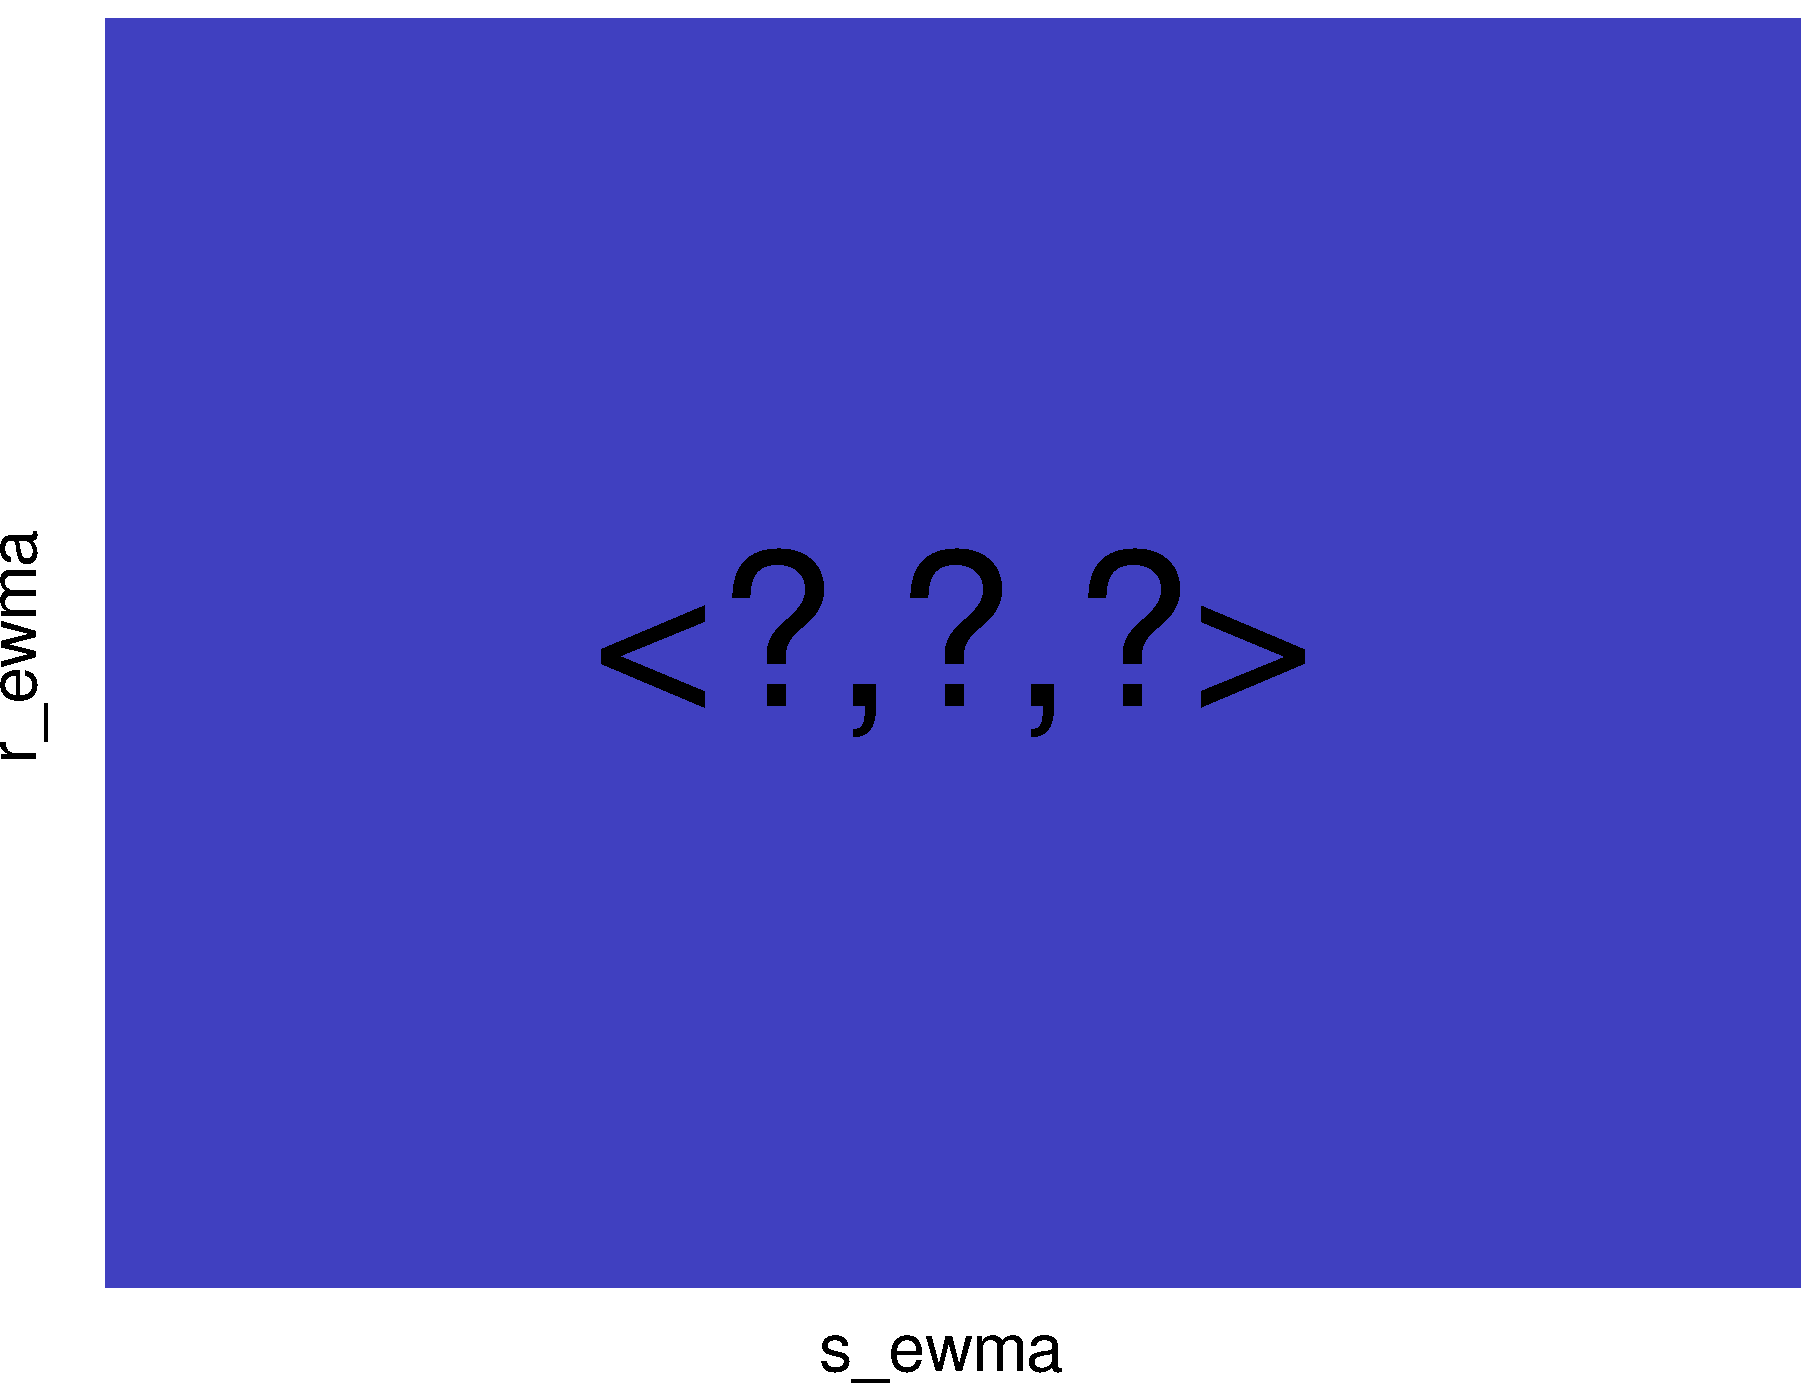
\includegraphics[width=9.25 cm]{remy-graph/graph/test0.pdf}

\end{centering}}
\only<2>{\frametitle{The best (single) action. Now split it on median.}
\begin{centering}
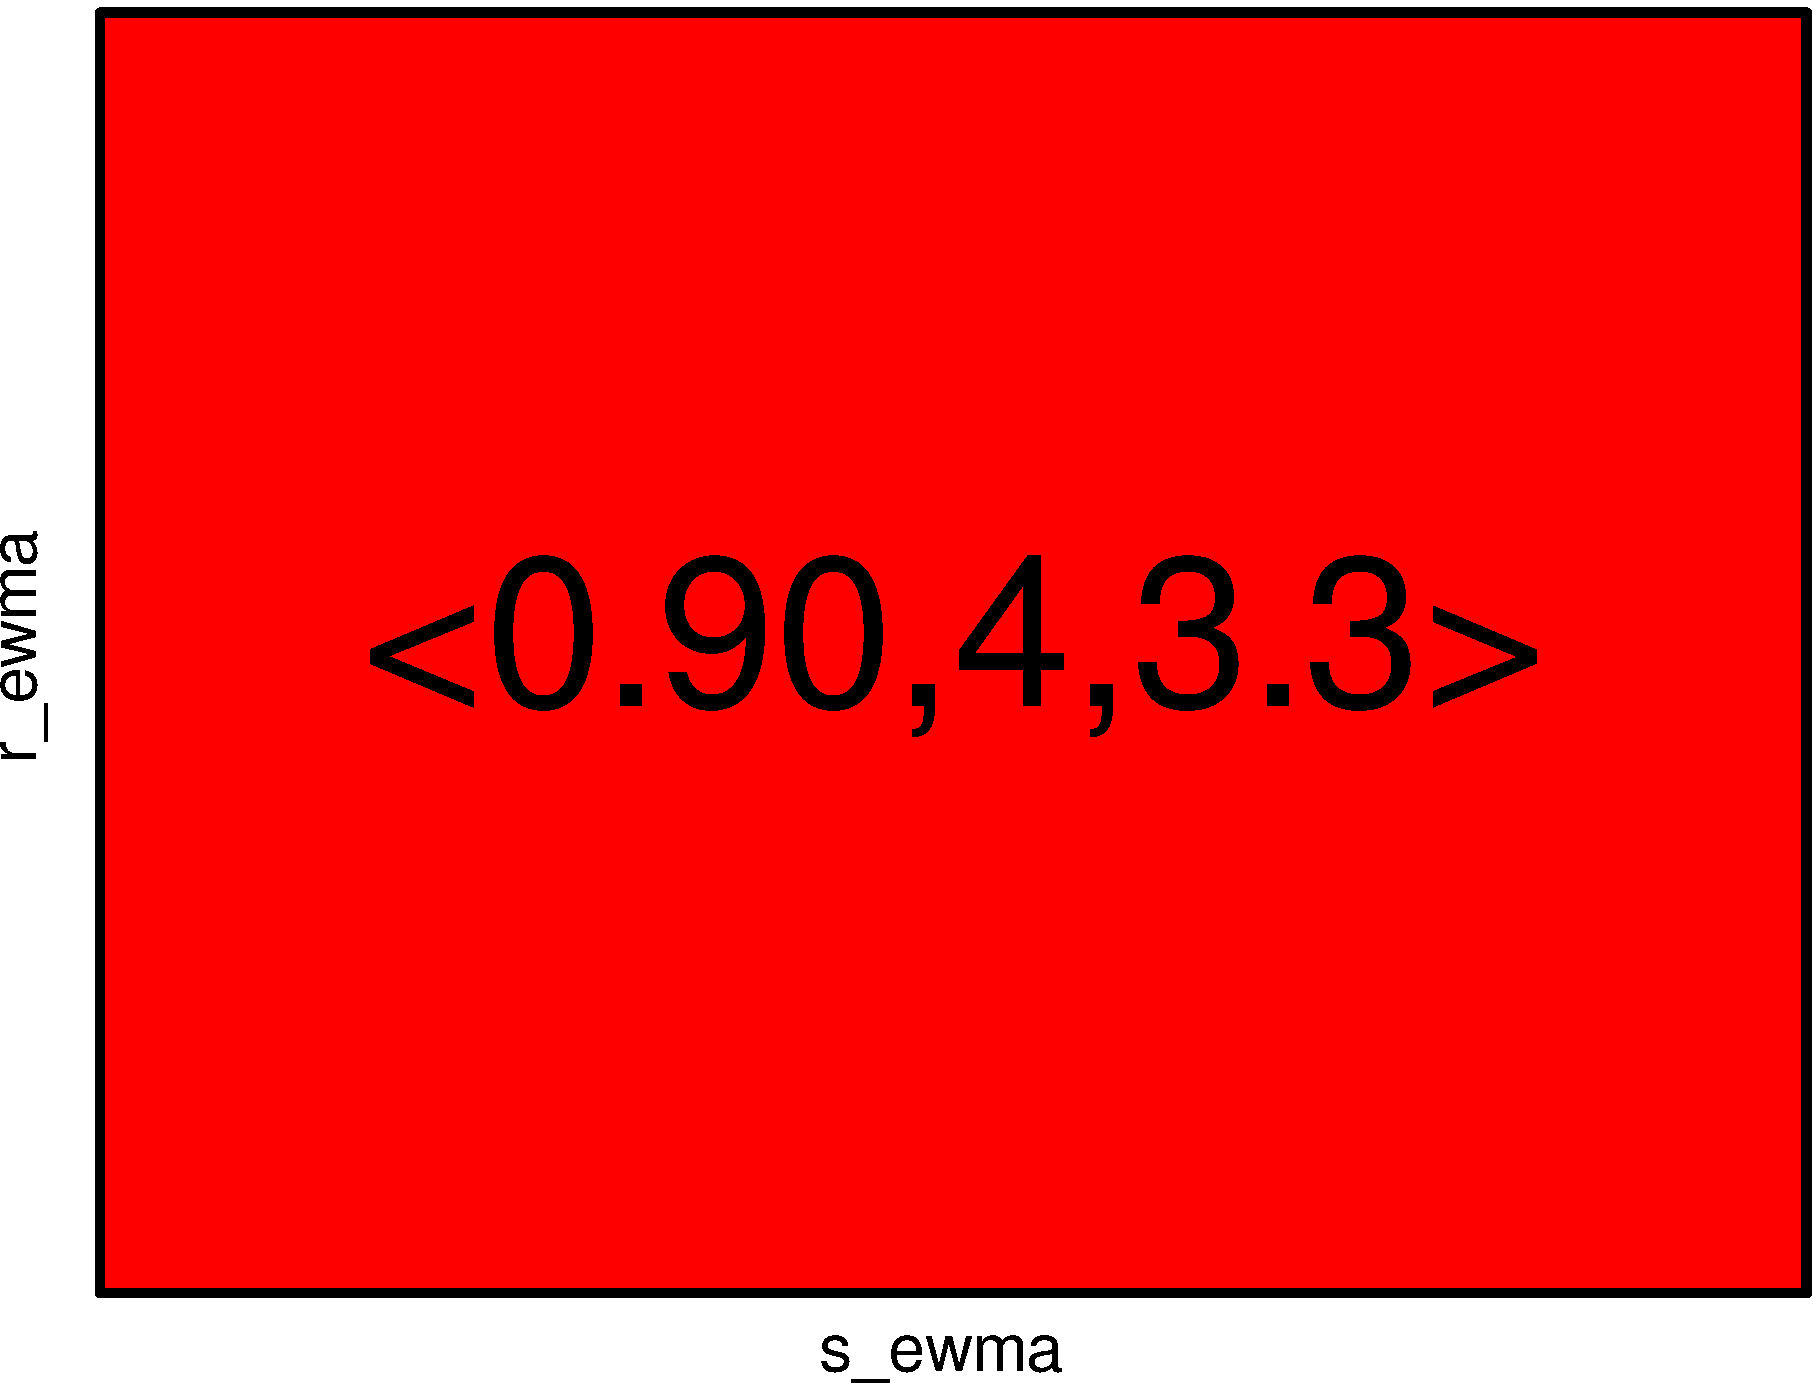
\includegraphics[width=9.25 cm]{remy-graph/graph/test1.pdf}

\end{centering}}

\only<3>{\frametitle{Simulate}
\begin{centering}
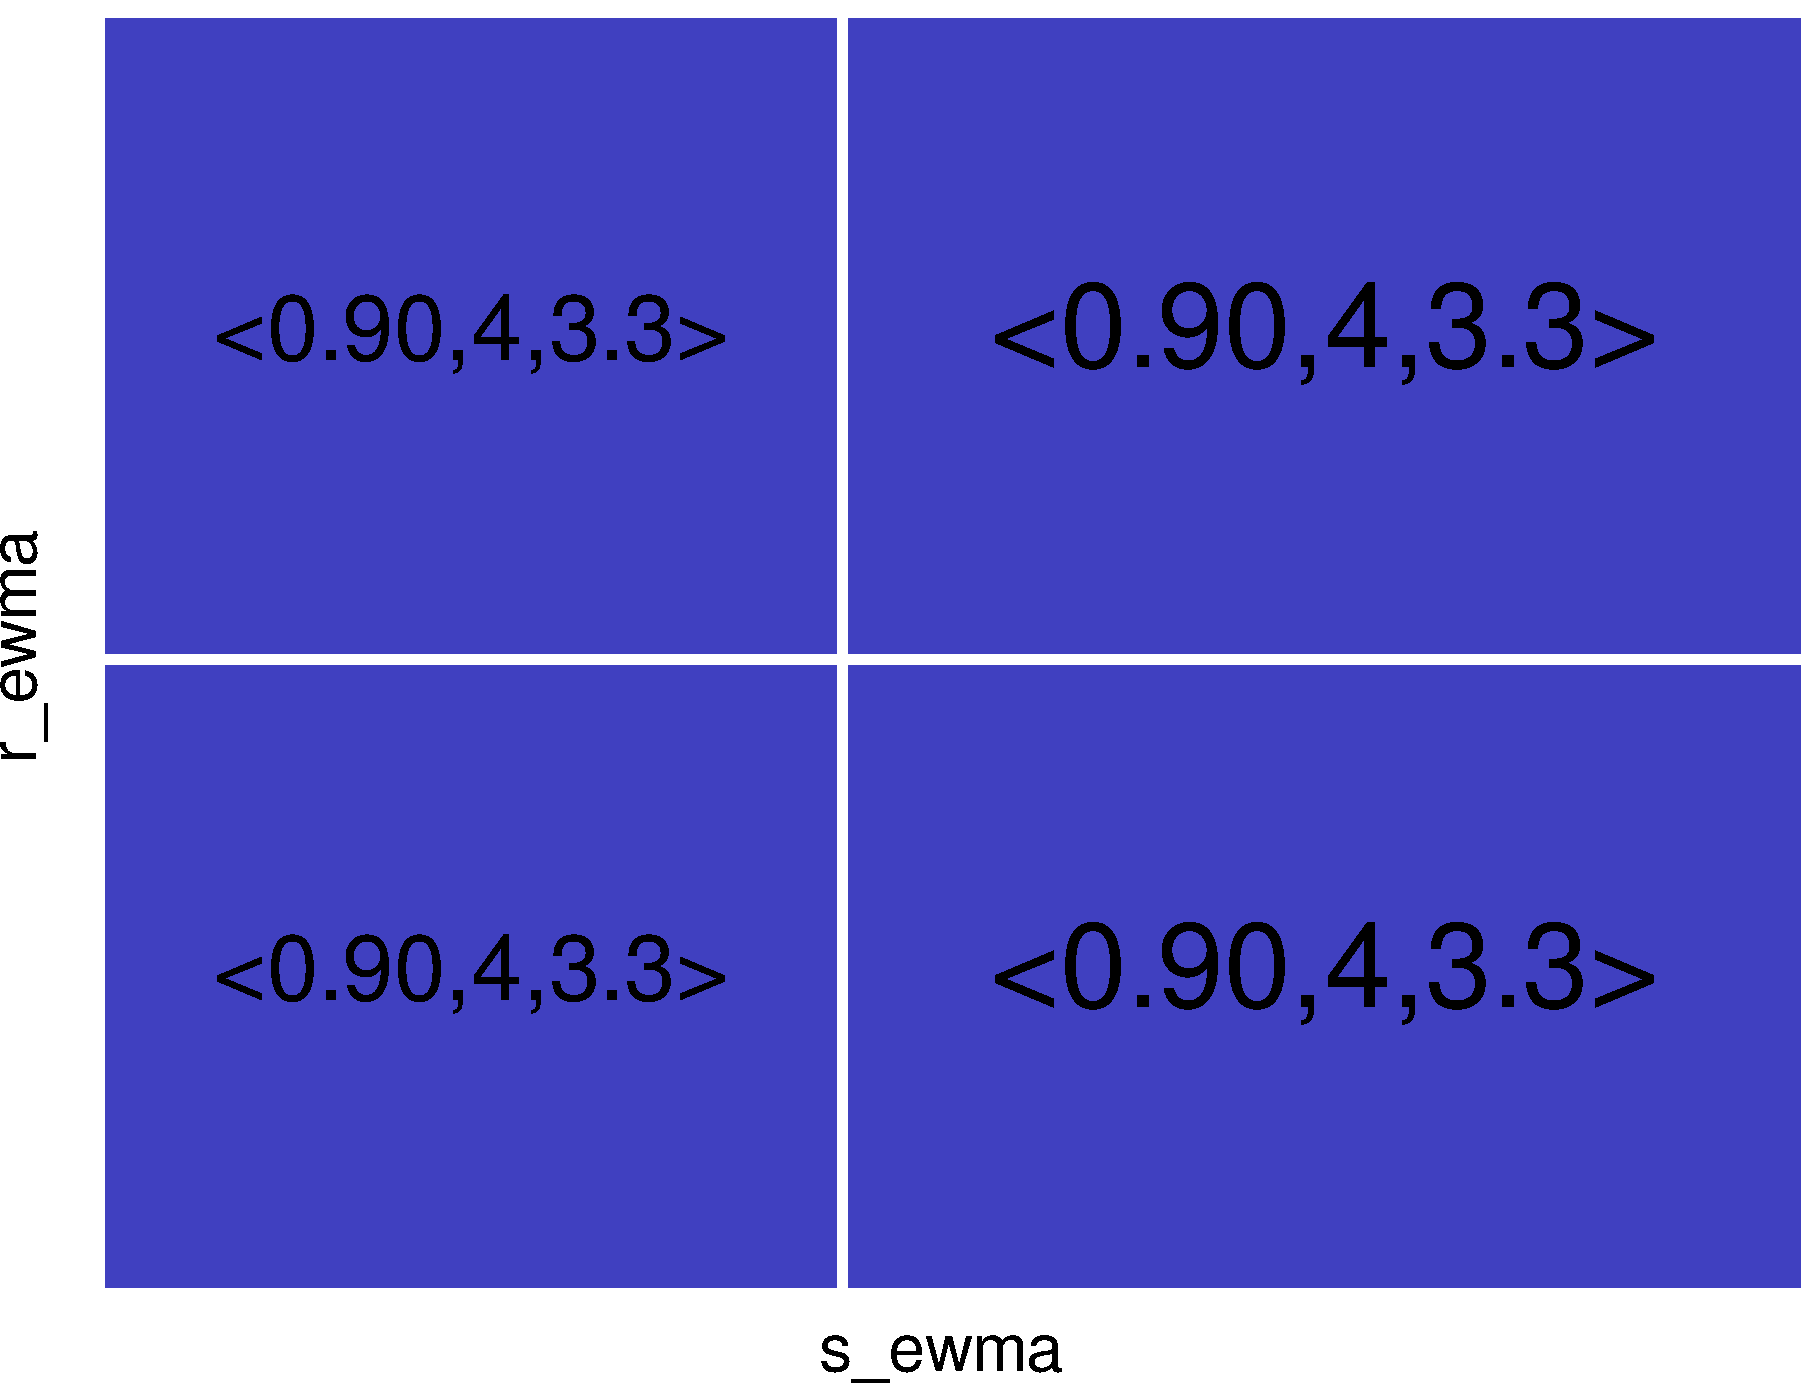
\includegraphics[width=9.25 cm]{remy-graph/graph/test2.pdf}

\end{centering}
}

\only<4>{\frametitle{Optimize each of the new actions}
\begin{centering}
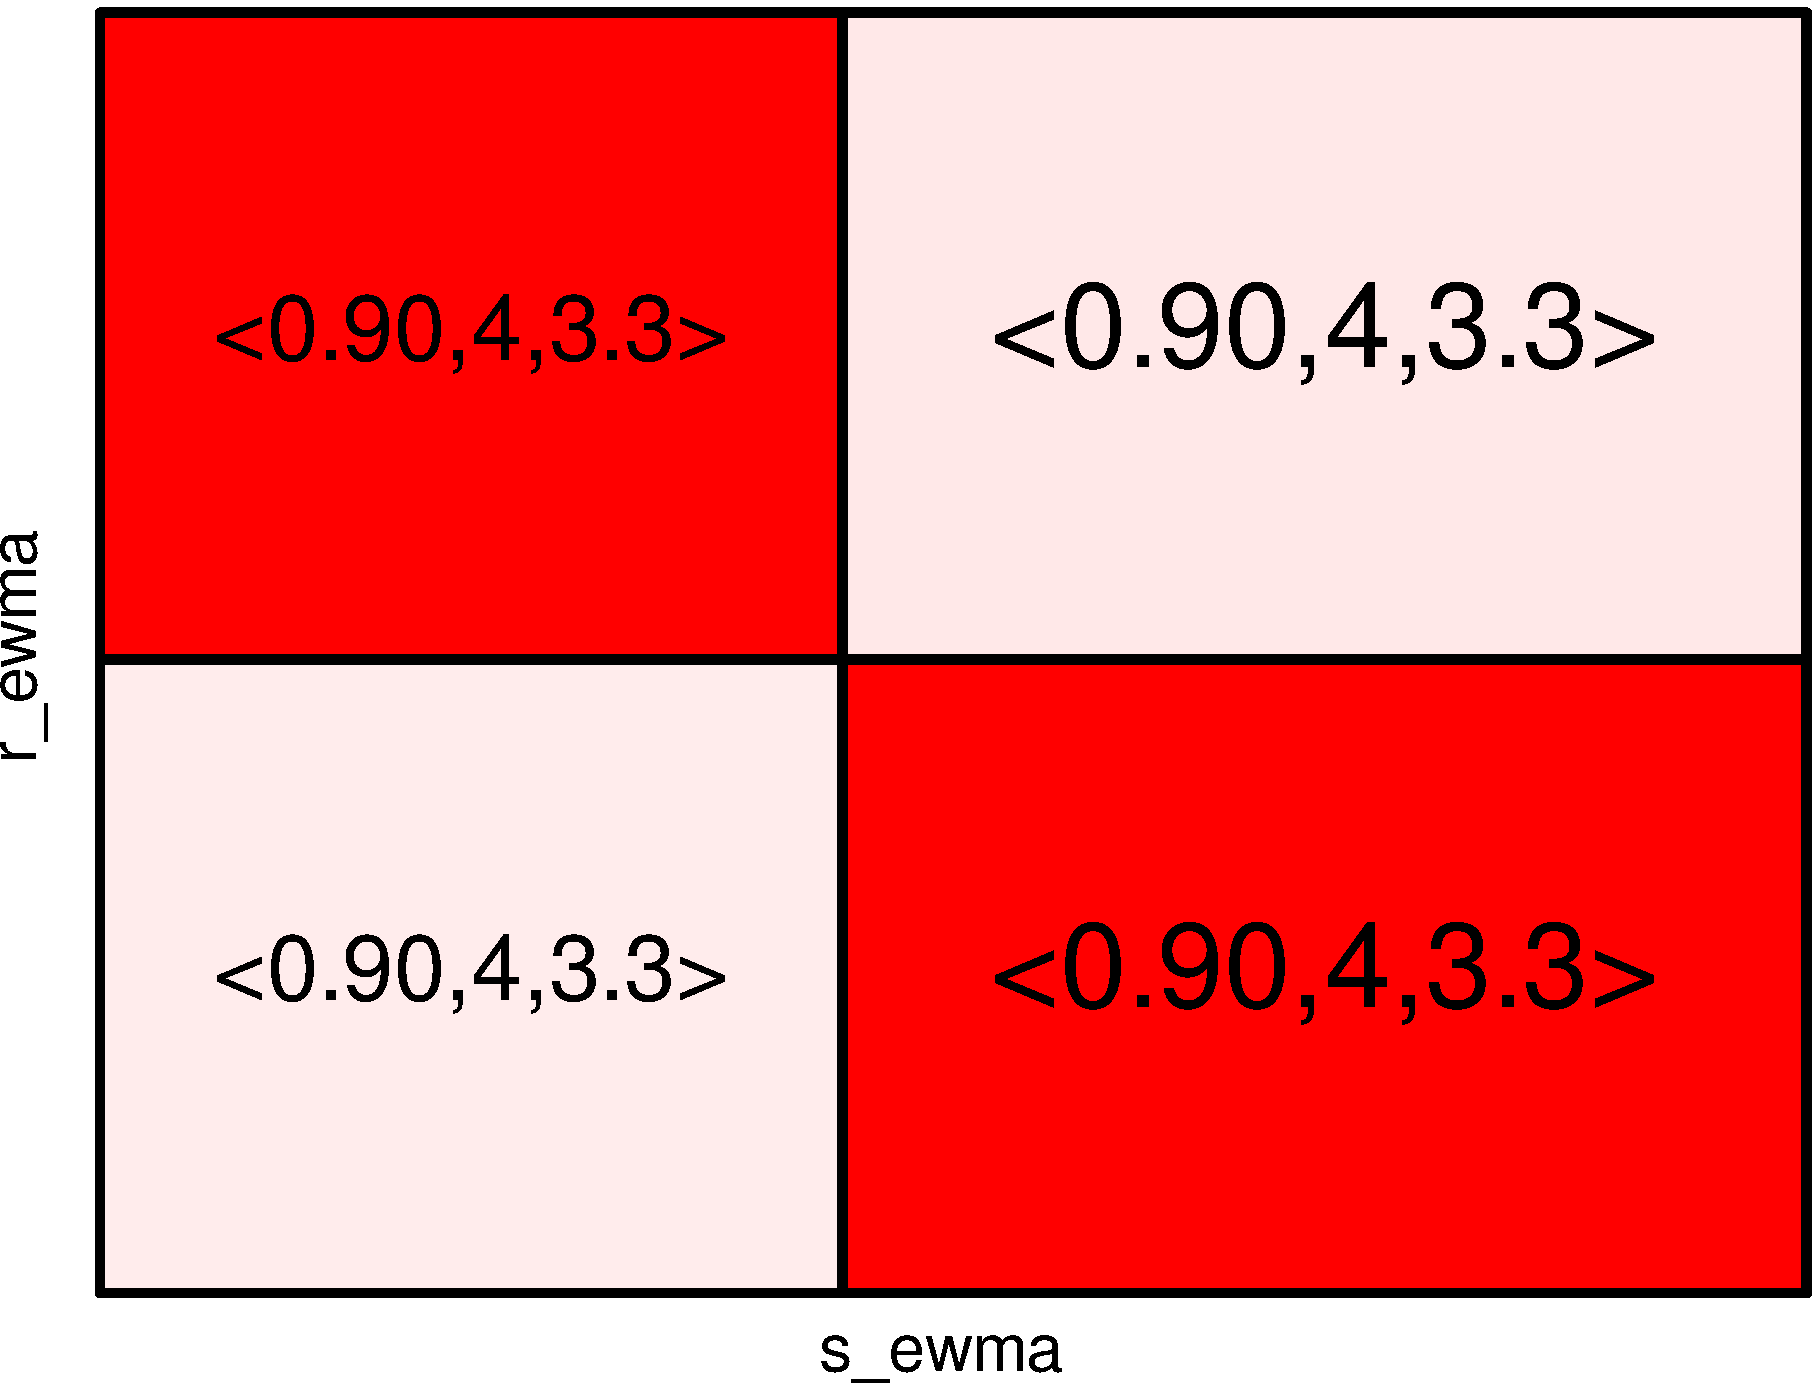
\includegraphics[width=9.25 cm]{remy-graph/graph/test3.pdf}

\end{centering}
}

\only<5>{\frametitle{Now split the most-used rule}
\begin{centering}
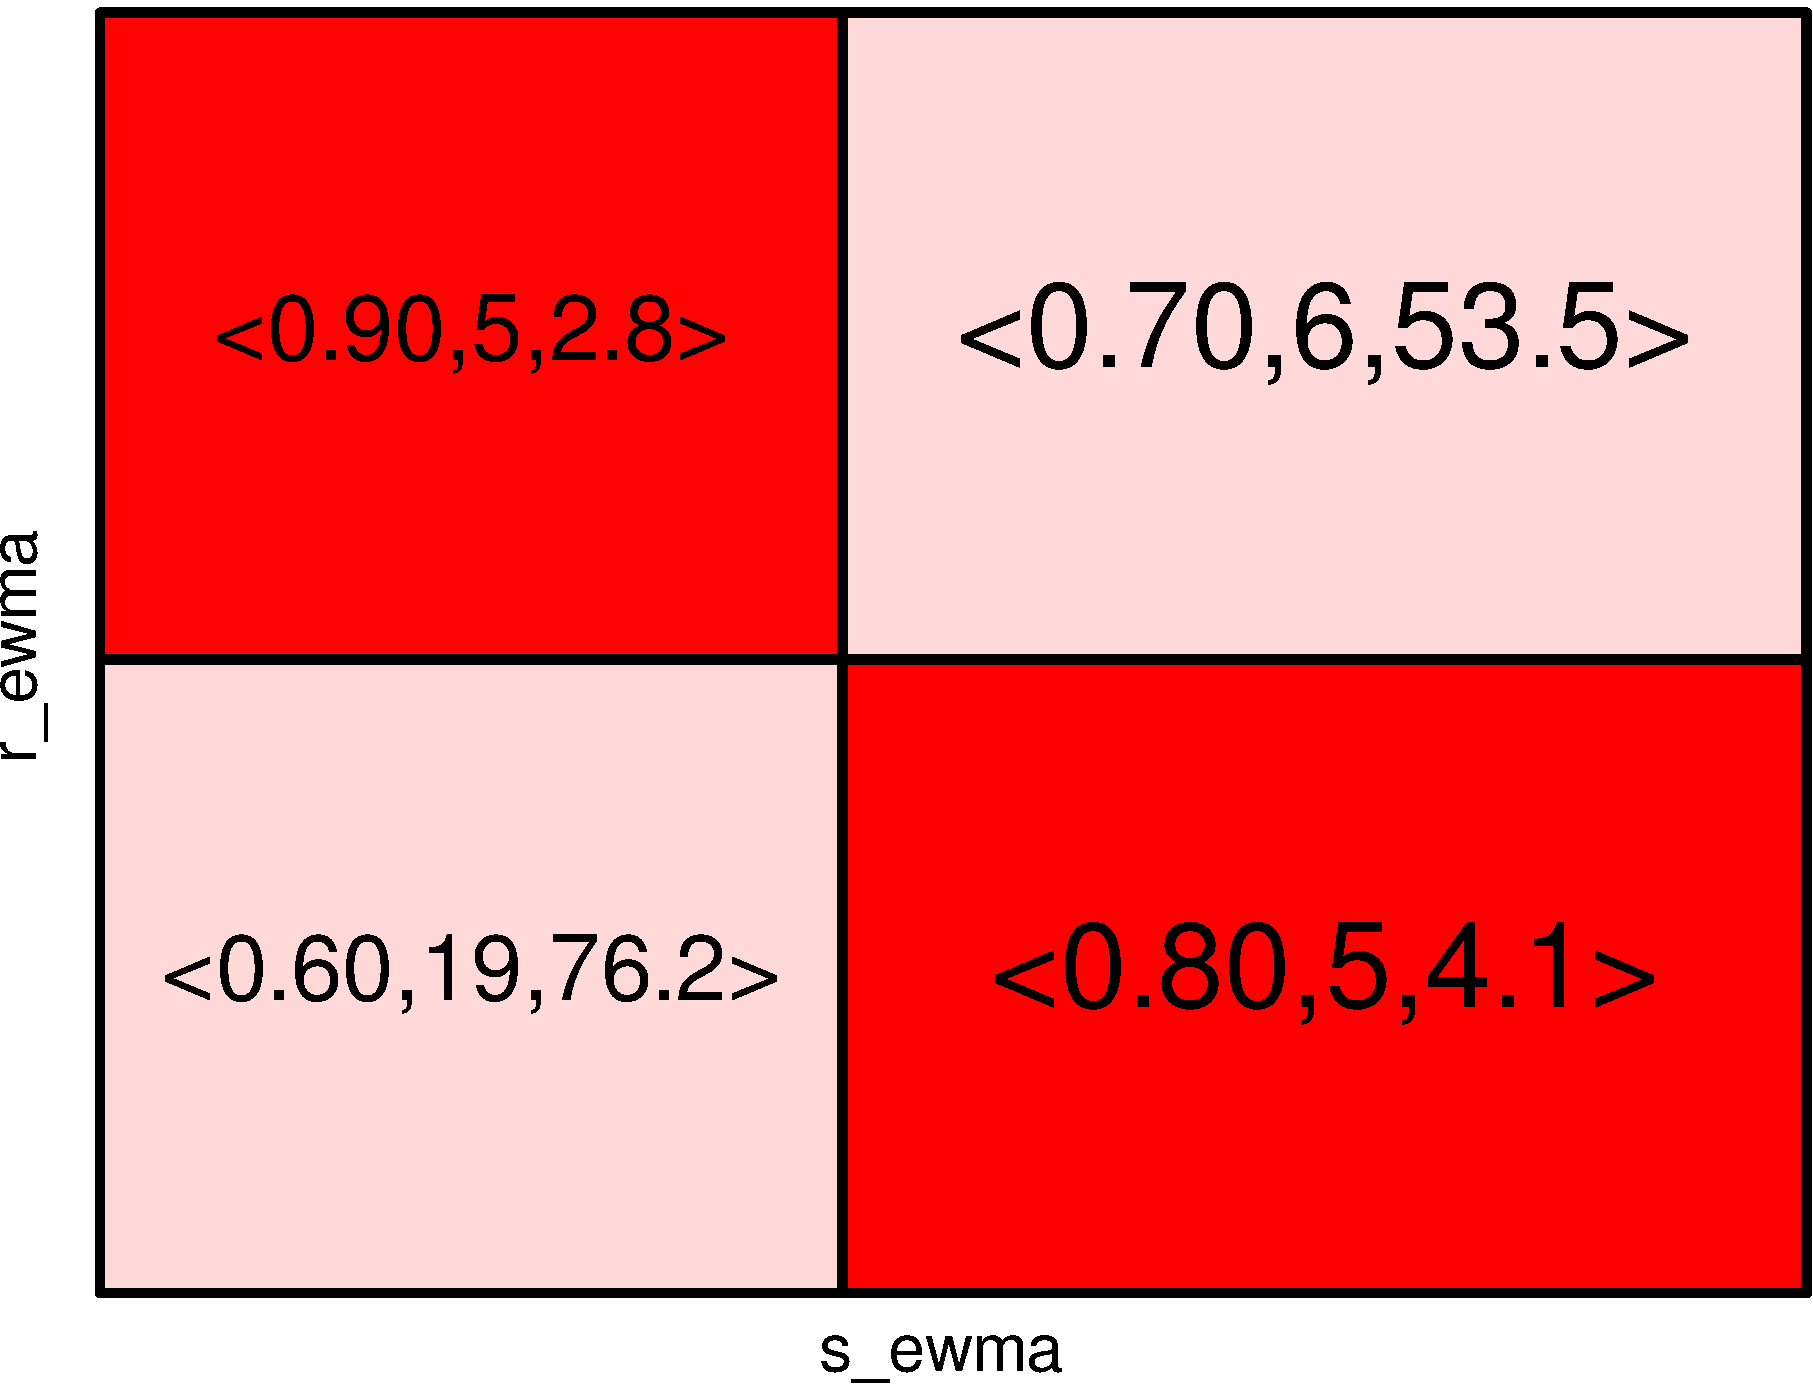
\includegraphics[width=9.25 cm]{remy-graph/graph/test4.pdf}

\end{centering}
}

\only<6>{\frametitle{Simulate}
\begin{centering}
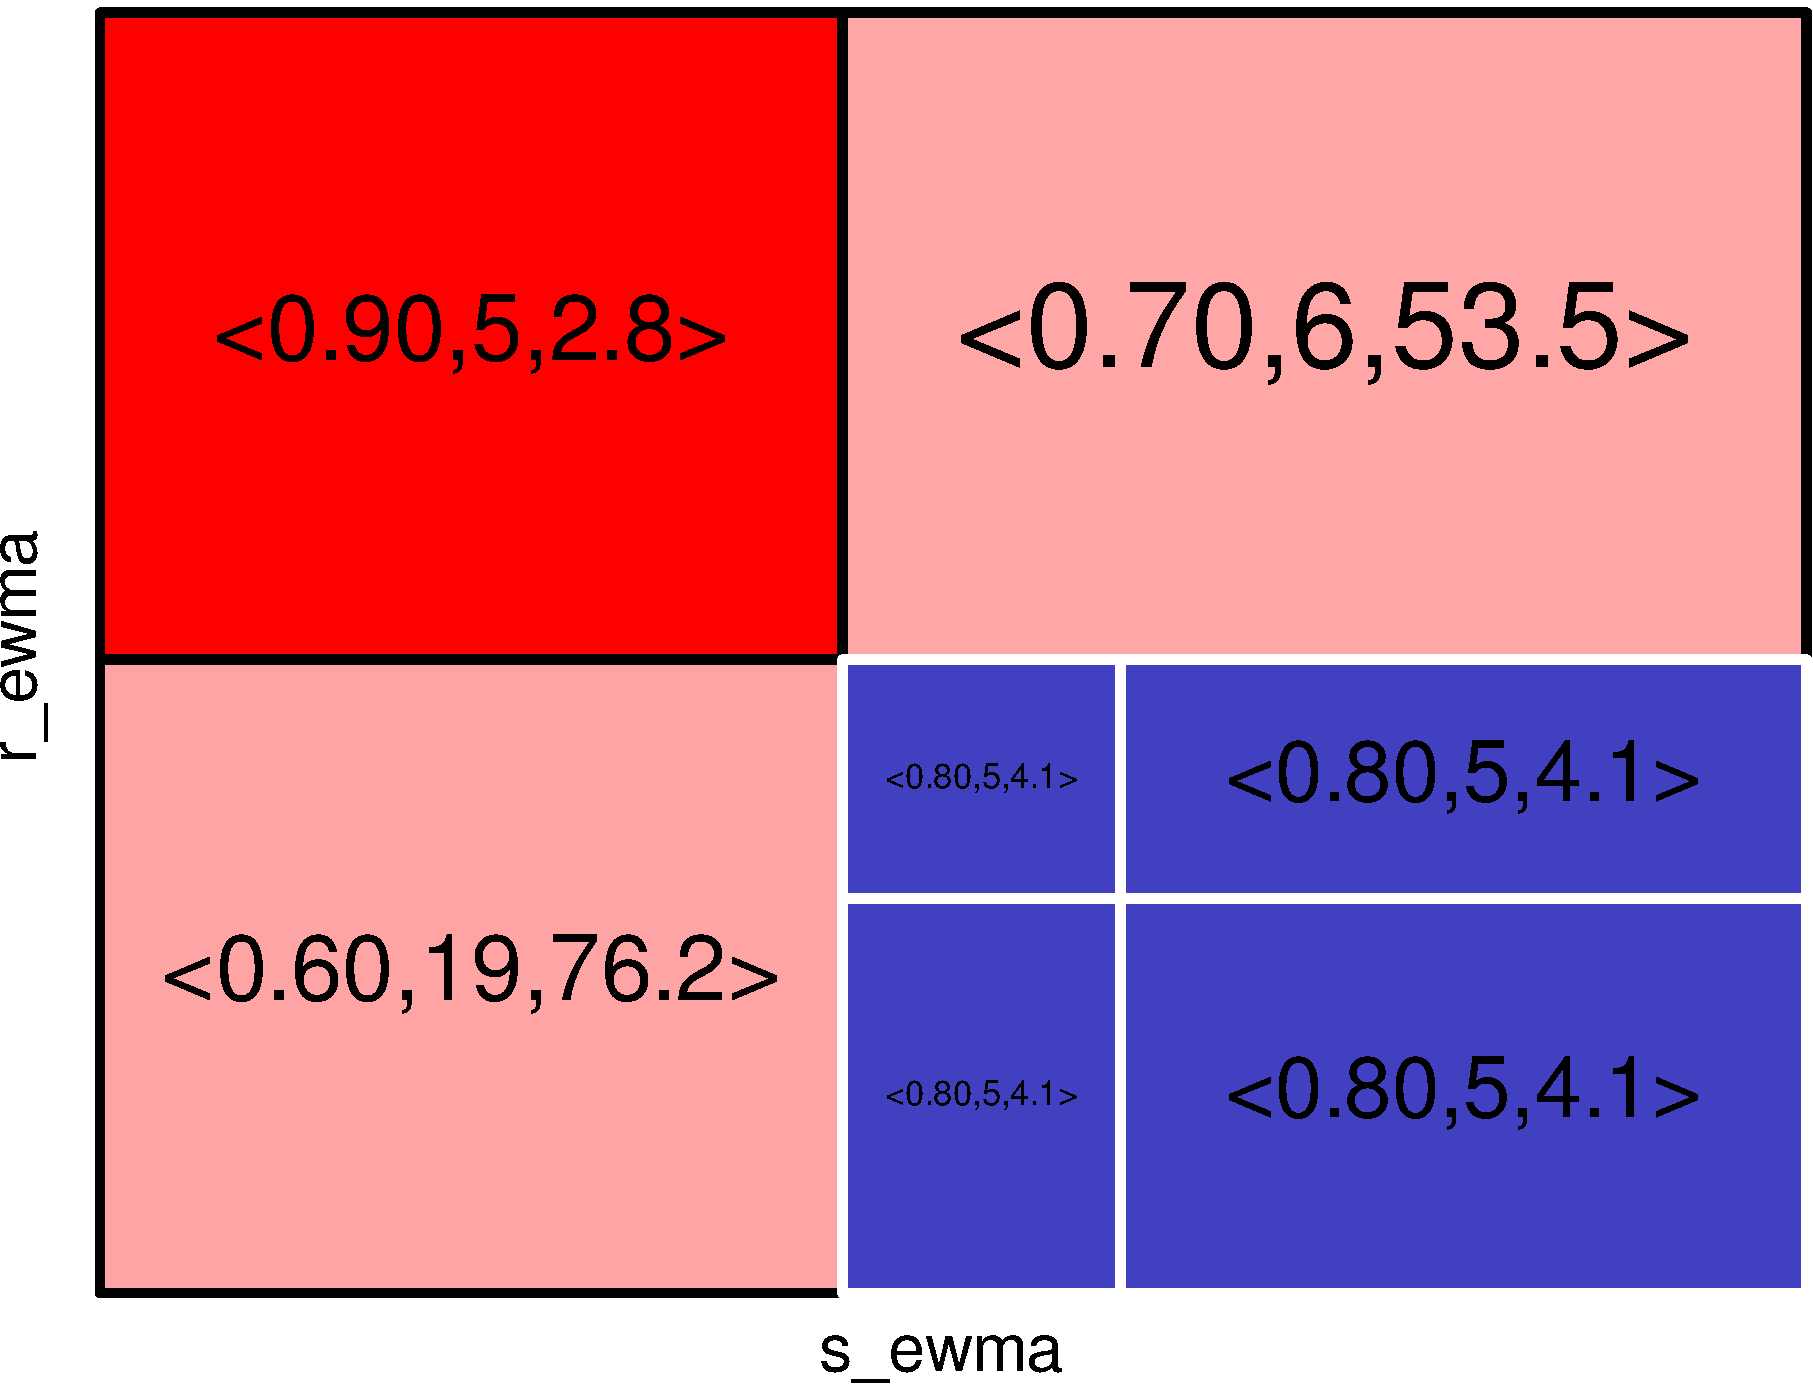
\includegraphics[width=9.25 cm]{remy-graph/graph/test5.pdf}

\end{centering}
}

\only<7>{\frametitle{Optimize}
\begin{centering}
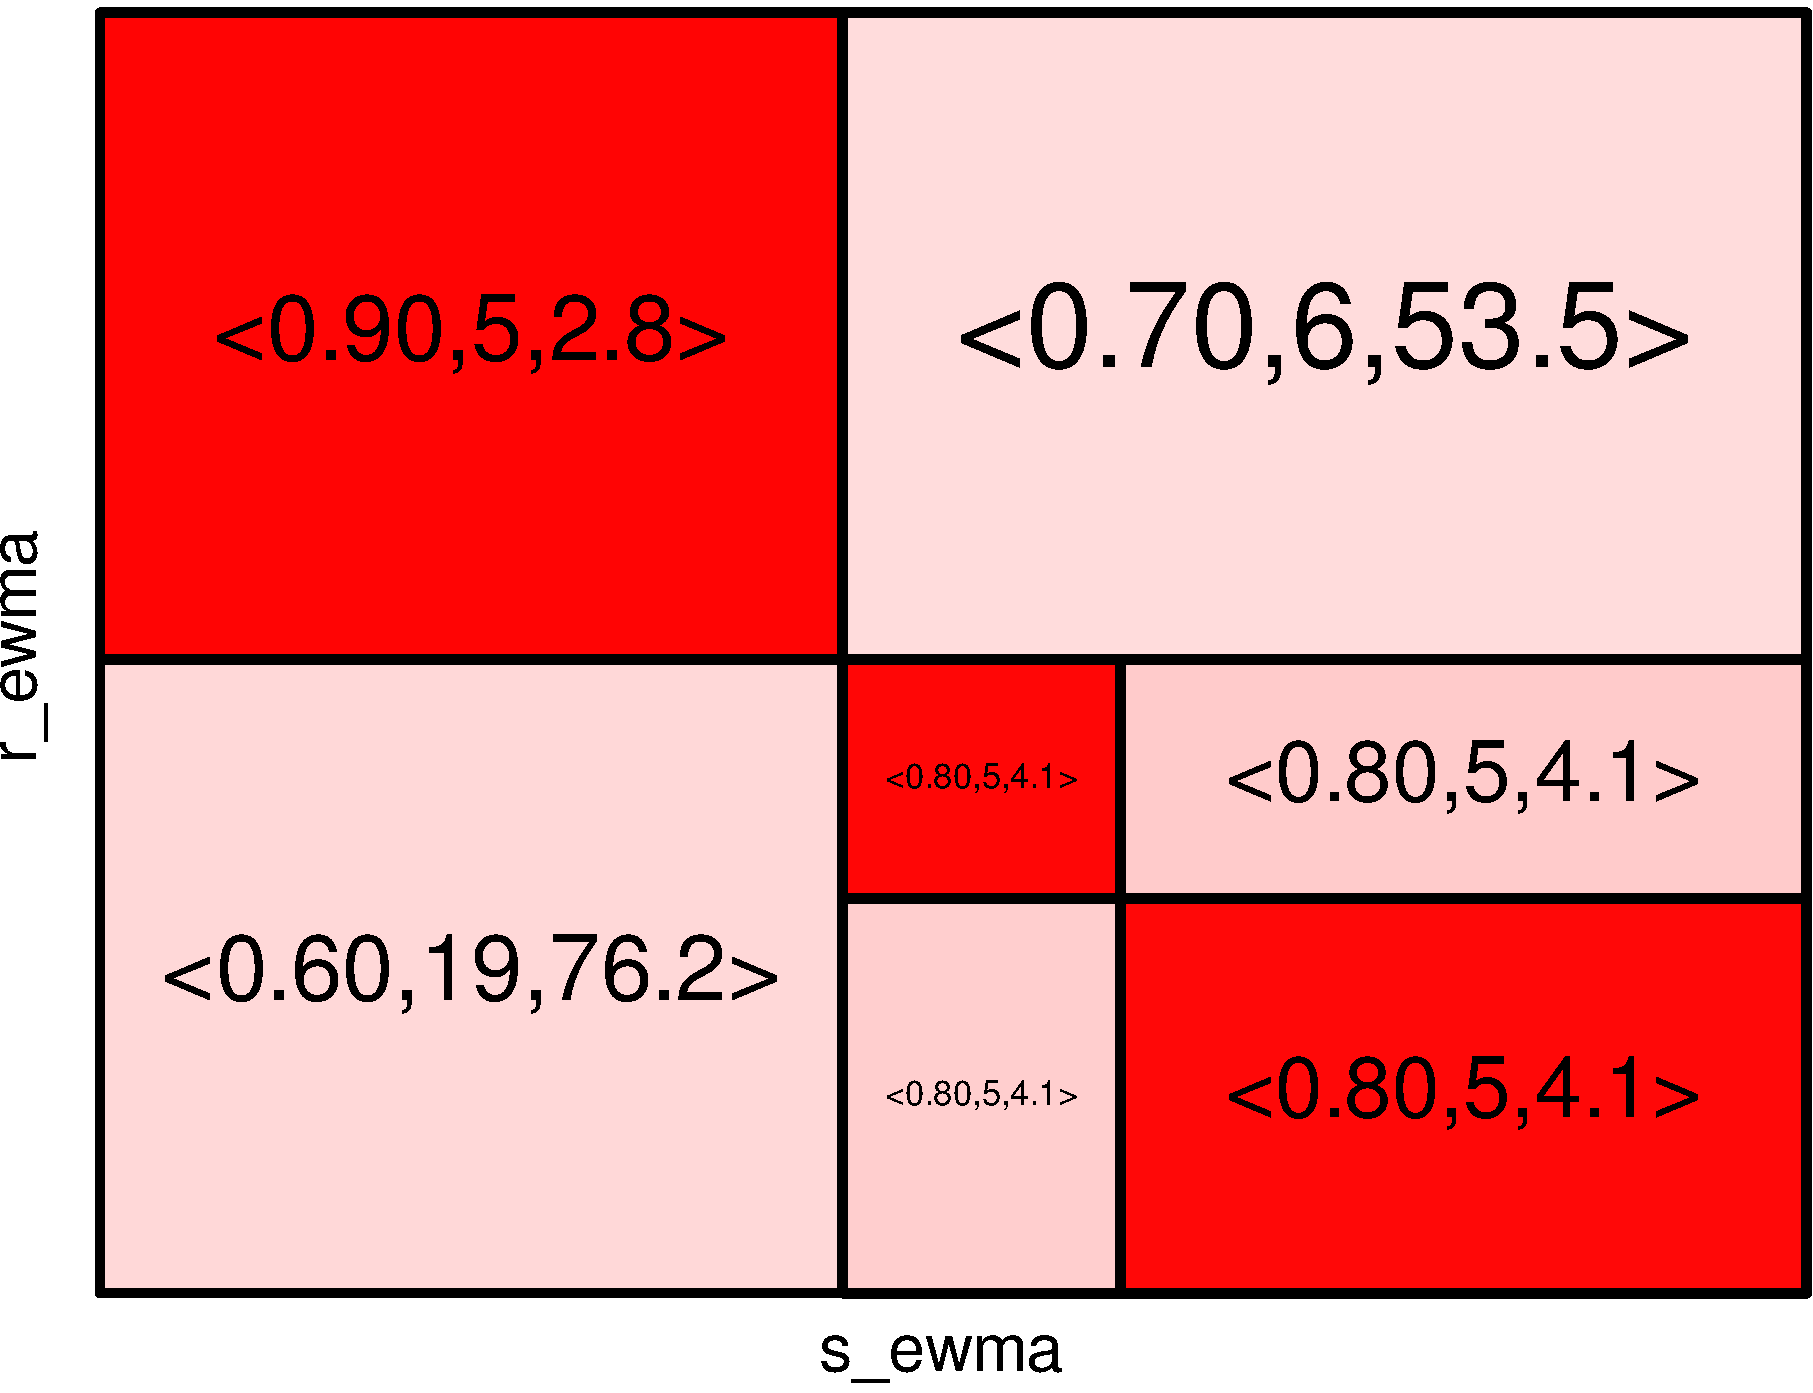
\includegraphics[width=9.25 cm]{remy-graph/graph/test6.pdf}

\end{centering}
}
\only<8>{\frametitle{Split}\begin{centering}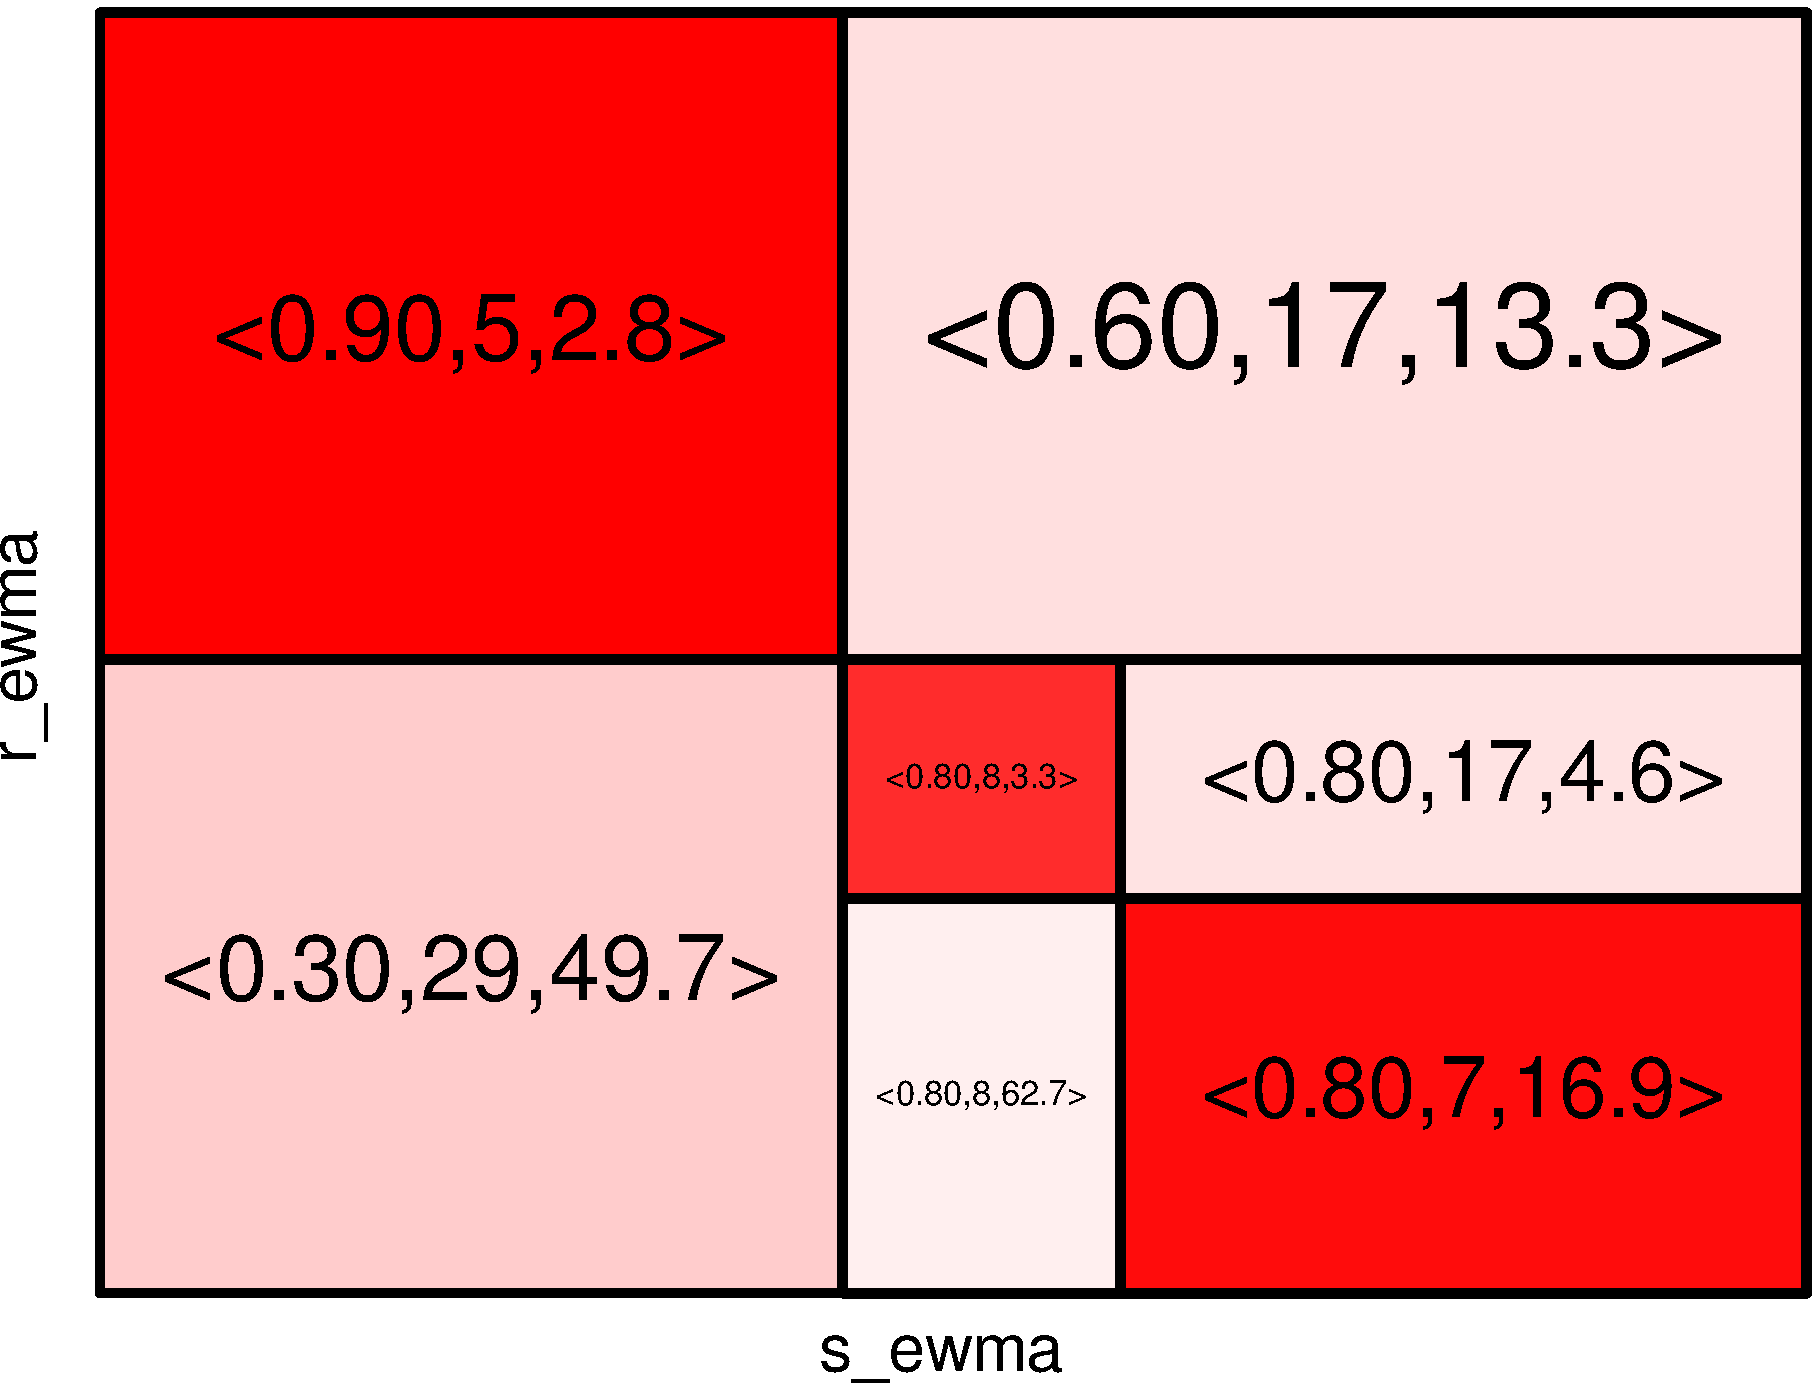
\includegraphics[width=9.25 cm]{remy-graph/graph/test7.pdf}

\end{centering}}

\only<9>{\frametitle{Simulate}\begin{centering}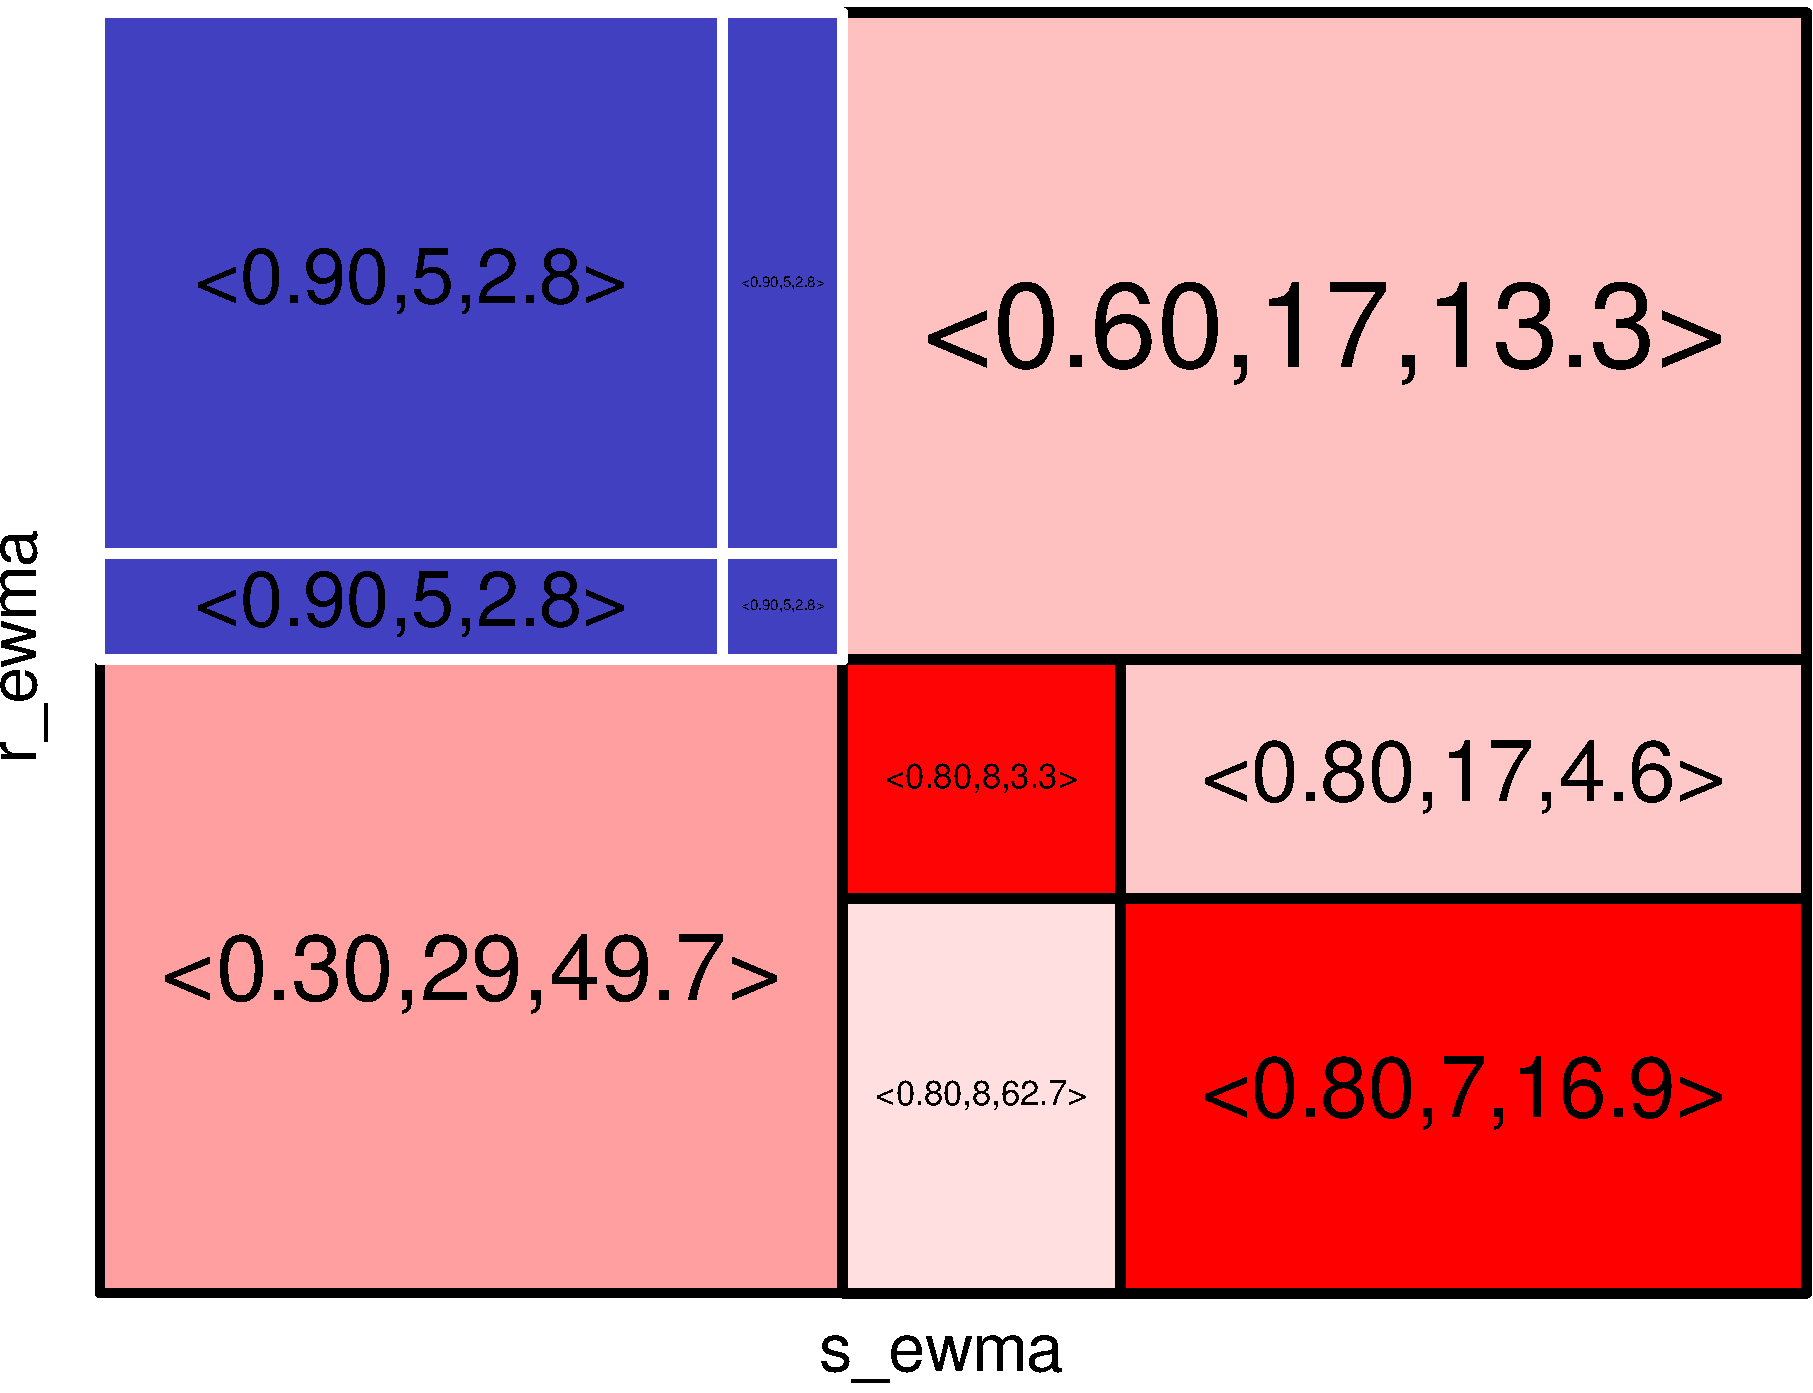
\includegraphics[width=9.25 cm]{remy-graph/graph/test8.pdf}

\end{centering}}

\end{frame}
